\documentclass[a4paper,12pt]{article}

% packages
\usepackage{amsmath}
\usepackage{amssymb}
\usepackage{graphicx}
\usepackage{fancyhdr}
\usepackage{hyperref}
\usepackage{float}



% Fancy header/footer settings
\pagestyle{fancy}
\fancyfoot[C]{}
\fancyfoot[R]{\thepage} % Right-align page number in the footer


% Title information
\title{AAD - Assignment 2}
\author{107474-Joseane Pereira \\
109050-Gabriel Costa \\
Universidade de Aveiro, DETI}
\date{\today}

\begin{document}

\begin{figure}
    \centering
    
\includegraphics[width=0.3\linewidth]{ua.pdf}
    \label{fig:enter-label}
\end{figure}
\maketitle
\newpage
\tableofcontents
\newpage
\section{Introduction}
This assignment focuses on the implementation and analysis of different 
accumulator designs in VHDL, including a single-cycle version, a pipelined 
version, and versions with shift functionality.


\section{Implementations}

\subsection{Single-Cycle Accumulator}
As suggested with the provided starting point, the basic accumulator was implemented in
\texttt{accumulator\_single\_cycle.vhd} with the following features:
\begin{itemize}
    \item Simple write and read ports
    \item Direct accumulation without pipelining
    \item Basic addition functionality
    \item Synchronous reset to initialize the accumulator
    \item Parameterizable data width for flexibility
\end{itemize}

The accumulator operates by reading an input value, adding it to the current stored value, and then writing the result back to the storage register in a single clock cycle. This design ensures minimal latency but does not support high-frequency operations due to the lack of pipelining.

\begin{figure}[H]
    \centering
    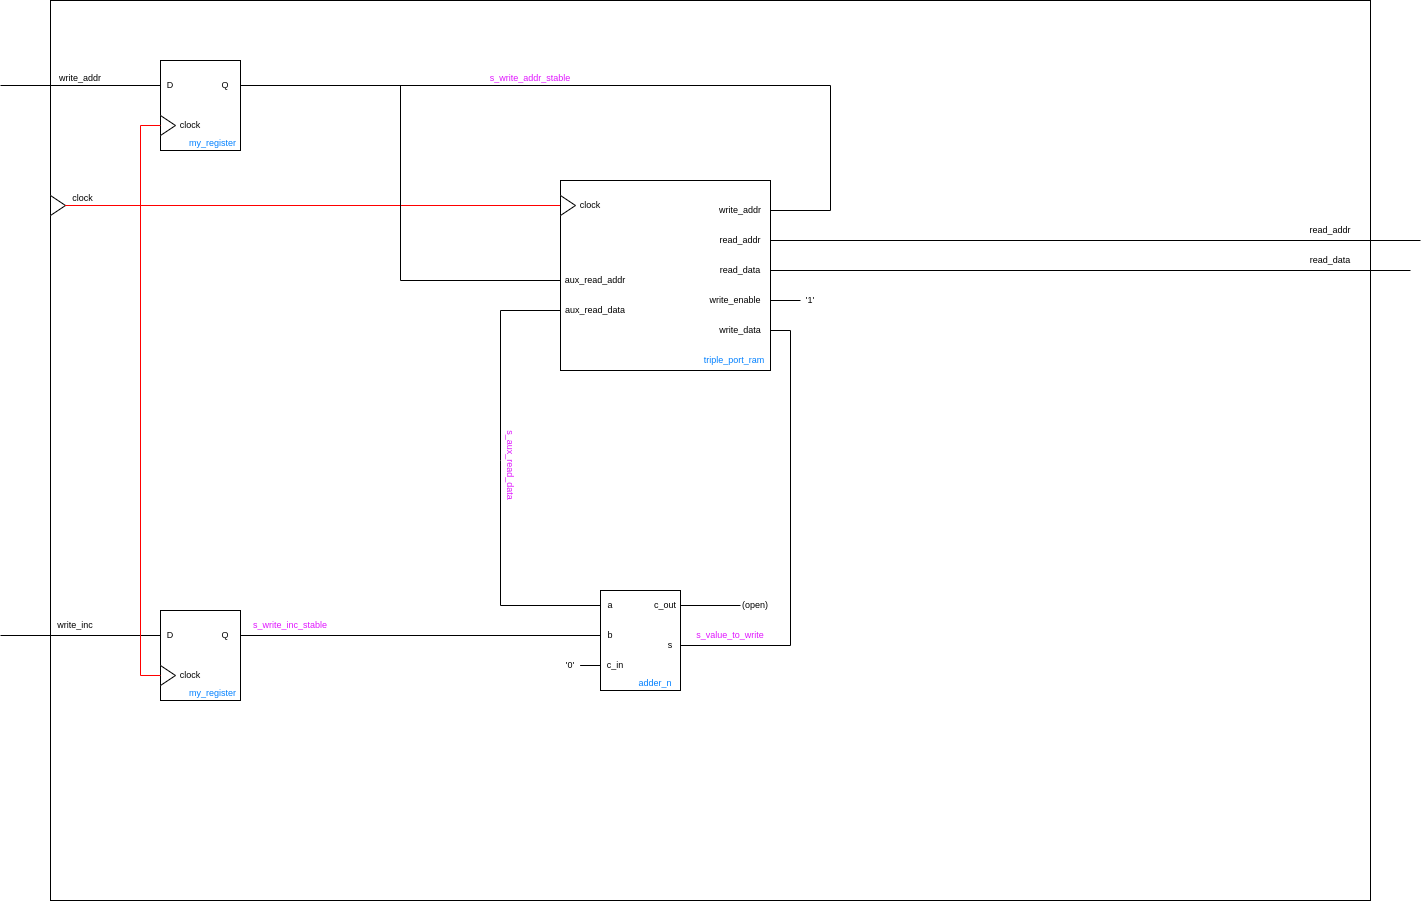
\includegraphics[width=1.0\linewidth]{accumulator_single_sycle.png}
    \caption{Single-cycle accumulator block diagram}
    \label{fig:single_cycle}
\end{figure}


\subsection{Pipelined Accumulator}
The pipelined version \texttt{accumulator\_pipeline.vhd} improves
 upon the basic design by:
\begin{itemize}
    \item Adding pipeline stages to improve throughput
    \item Using registers to stabilize signals
    \item Implementing hazard detection
\end{itemize}

\begin{figure}[H]
    \centering
    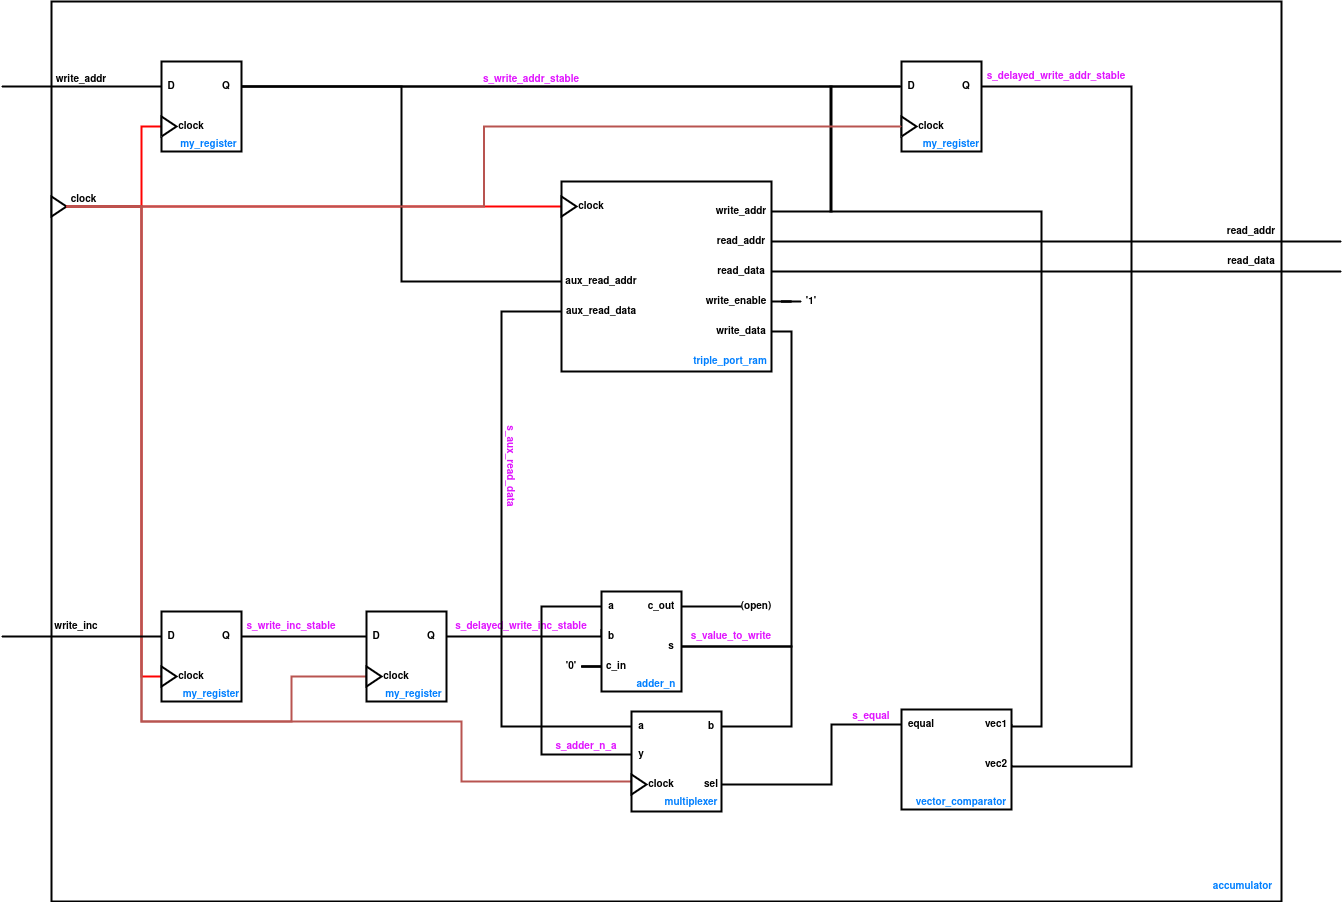
\includegraphics[width=1.0\linewidth]{accumulator_pipeline.png}
    \caption{Pipelined accumulator block diagram}
    \label{fig:pipeline}
\end{figure}

\subsection{Shift Accumulator}
We implemented a version of the accumulator using a barrel shifter for both the pipelined and single cycle versions (\texttt{shift\_accumulator\_pipeline.vhd} and \texttt{shift\_accumulator.vhd}), both of which improve upon the basic design by:
\begin{itemize}
    \item Dynamic shift operations on input data
    \item Configurable shift amounts
    \item Integration with the accumulation logic
\end{itemize}

The shift accumulator design leverages a barrel shifter to perform dynamic shift operations on the input data. This allows for efficient manipulation of data bits, which is crucial for various digital signal processing tasks. The configurable shift amounts enable the design to be flexible and adaptable to different requirements, making it suitable for a wide range of applications.

In the single cycle version, the shift and accumulation operations are performed within a single clock cycle. This design is optimized for scenarios where speed is critical, and the simplicity of the control logic is a priority. The block diagram in Figure \ref{fig:shift} illustrates the architecture of the single cycle shift accumulator.

\begin{figure}[H]
    \centering
    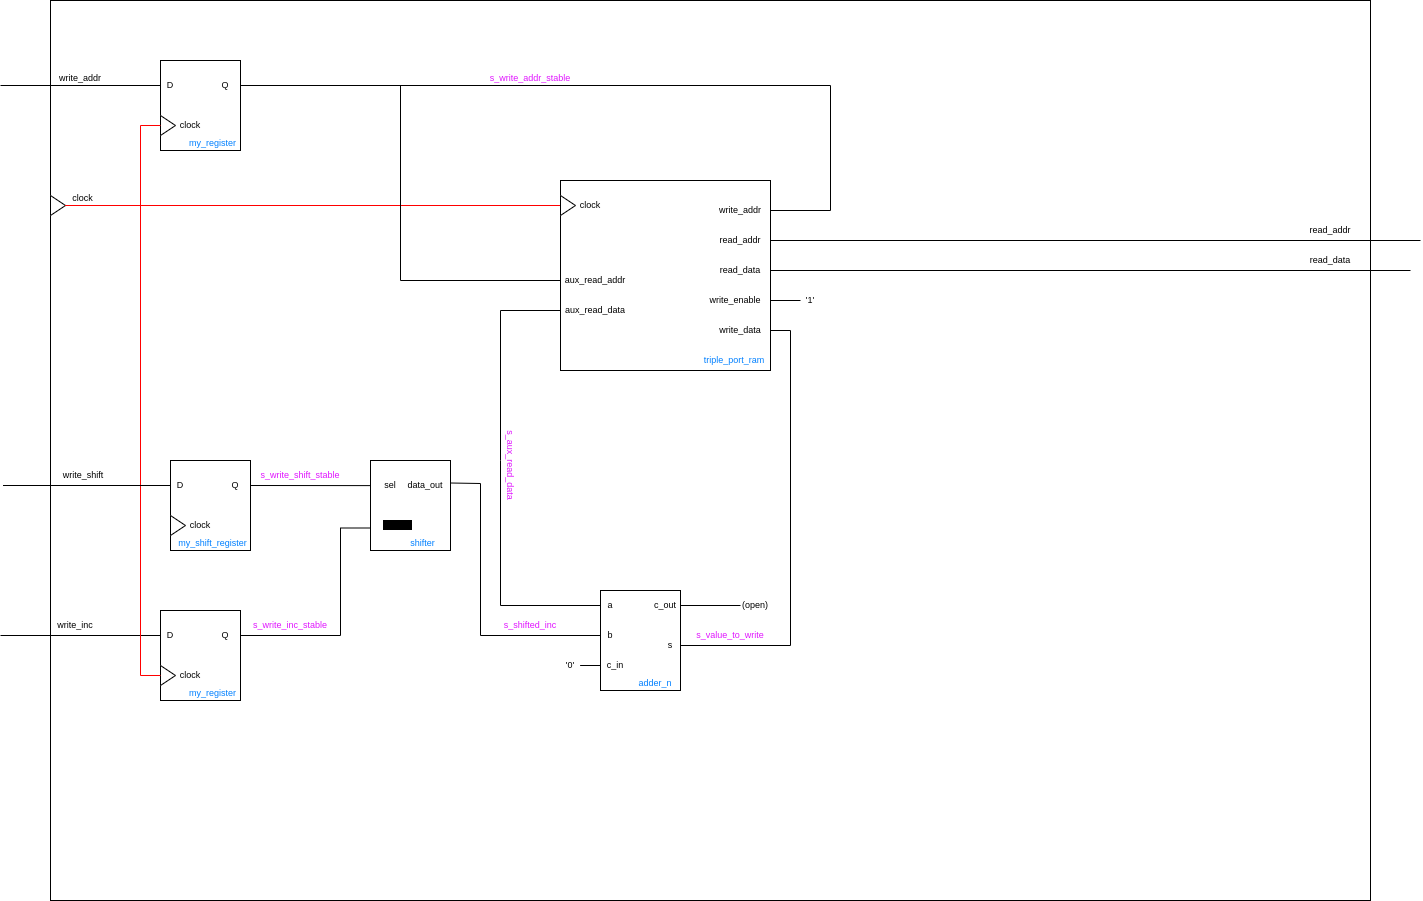
\includegraphics[width=1.0\linewidth]{accumulator_shift_single_sycle.png}
    \caption{Shift accumulator single cycle block diagram}
    \label{fig:shift}
\end{figure}

For the pipelined version, the design is divided into multiple stages, allowing for higher clock frequencies and improved throughput. Each stage of the pipeline performs a portion of the shift and accumulation operations, enabling the design to handle higher data rates. This is particularly beneficial in applications where large volumes of data need to be processed efficiently. The block diagram in Figure \ref{fig:shift_pipeline} shows the architecture of the pipelined shift accumulator.

\begin{figure}[H]
    \centering
    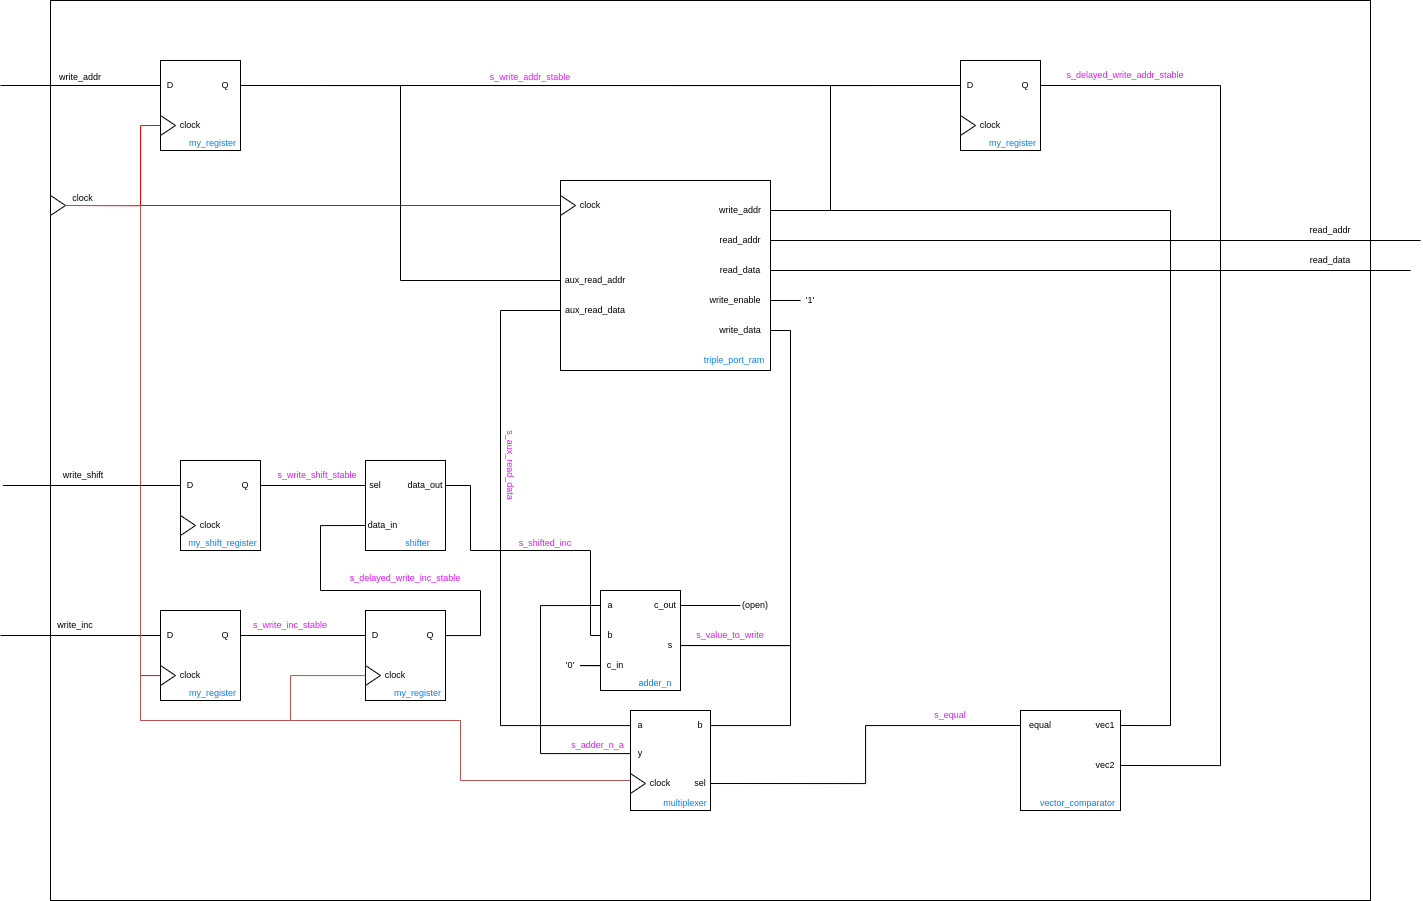
\includegraphics[width=1.0\linewidth]{accumulator_shift_pipeline.png}
    \caption{Shift accumulator pipeline block diagram}
    \label{fig:shift_pipeline}
\end{figure}

Overall, the shift accumulator designs provide a robust and flexible solution for data manipulation and accumulation tasks, with the pipelined version offering enhanced performance for high-speed applications.

\section{Components}
Some of the Components were provided by the professor, and some were 
implemented by us.
Key components used in the designs include:
\begin{itemize}
    \item Triple Port RAM for memory storage
    \item Registers for signal stabilization
    \item Adder N for arithmetic operations
    \item Shifter for shift operations
    \item Vector Comparator for address comparison
\end{itemize}

\section{Testing}
Testing was performed using:
\begin{itemize}
    \item GHDL simulator
    \item VCD waveform generation
    \item A provisded testbench for the single-cycle accumulator adapted for the pipelined and shift versions
\end{itemize}

\section{Results and Analysis}
    % Results and analysis
    %figue waveform
\begin{figure}[H]
    \centering
    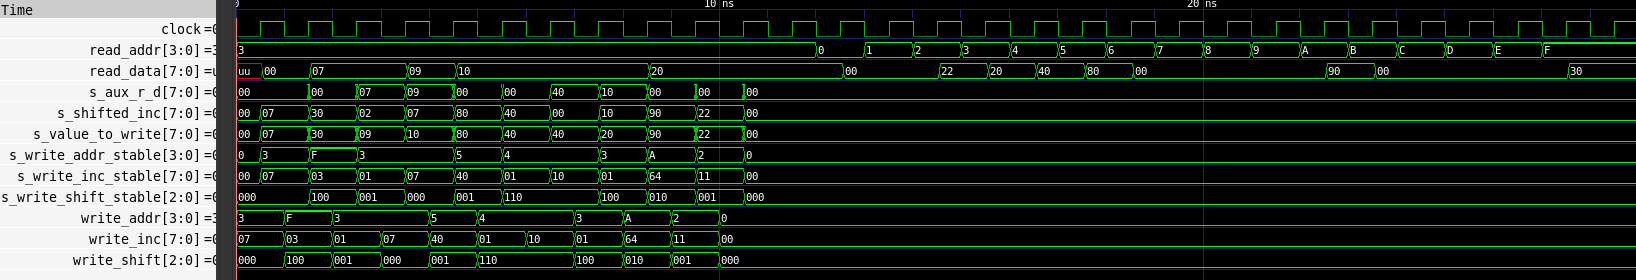
\includegraphics[width=0.8\linewidth]{waveform.png}
    \caption{Waveform of the single-cycle accumulator testbench}
    \label{fig:waveform}
\end{figure}

\ref{fig:waveform} shows the waveform generated by the testbench for the single-cycle accumulator. The testbench was adapted for the pipelined and shift versions, and the results were similar. The shift accumulator was tested with different shift amounts, and the results were as expected.

\section{Conclusions}
This project demonstrated the design and analysis of various accumulator architectures in VHDL: single-cycle, pipelined, and shift-based. The single-cycle design offered simplicity and minimal latency but was limited in scalability for high-speed operations. The pipelined accumulator addressed this by improving throughput and enabling higher clock frequencies. The shift accumulator added flexibility with dynamic shift operations, making it suitable for data-intensive applications.

Testing validated the functionality of all designs, with each meeting expected performance criteria. Overall, the project highlighted the trade-offs between simplicity, speed, and flexibility in digital system design. Future improvements could focus on optimizing power and area efficiency while exploring additional features.
\end{document}